
% \section*{Contemplación y EDGES} % Espacio para hablar del proyecto de (acomplete) de Dorian

\iffalse
\begin{itemize}
\item Distopía
\item domo 
\item Underborders
\item Milena y Concepción
\item setInterval()
\item Contemplación del fin del Mundo
\item sistemas mixtos
\item espacio y performance fusionados en Contemplación
\end{itemize}
\fi

% \color{BlueViolet}

\textit{Distopía}, \textit{NLXS + NK}, \textit{Interconexión}, \textit{setInterval()} y \textit{La Contemplación del Fin del Mundo} fueron los eventos realizados en el marco del Ciclo de Conciertos Audiovisuales \textit{EDGES}. Una de las primeras reflexiones partió de las distinciones más inmediatamente identificables con estos espacios: mundos virtuales / mundos reales, materialidad / inmaterialidad. Consideramos que procesos como los de \textit{Panorama} transitan entre la extensión de la fisicalidad hacia la virtualidad\footnote{``la trascendencia de la fisicalidad del mundo virtual nos permite extender nuestro modo de operación en el mundo físico. Nuevas formas de viaje, una nueva forma de comunicación, una nueva forma de operación, un nuevo medio de expresión" \citep[pp.~49]{cyberspace}}  y la reconfiguración de la materialidad\footnote{``el arte no solamente podría ser performeado en el plano sensorial, sino también en el plano inteligible. Las estéticas de la participación y la constitución de los medios digitales podrían intepretarse como la continuación de algunos de esos principios." \citep[pp.~190]{andreasosa}} de cara al giro digital que posibilita la continuación y contraposición estéticas y formas de organización social. 

\color{black}


%\begin{figure}[H]
%  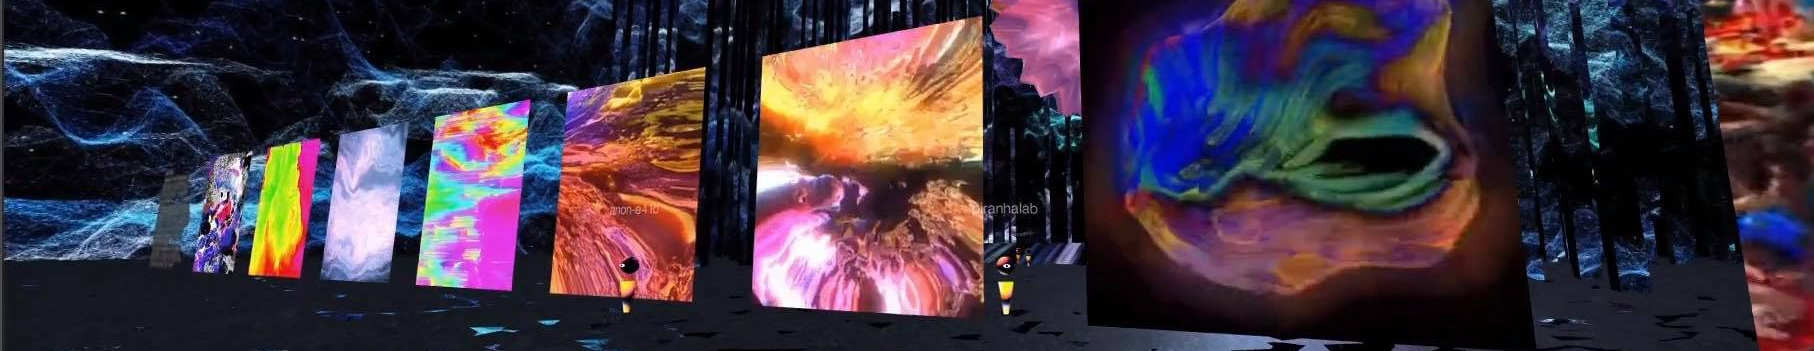
\includegraphics[width=\textwidth]{img/distopia.png}
%  \caption{EDGES Distopía. Imágenes: LVSTVCRV}
%\end{figure}

\textit{La Contemplación del Fin del Mundo} fue el último evento de EDGES. Consideramos que fue el punto de coincidencia entre las reflexiones anteriormente enunciadas y su realización tecnológica. \textit{La contemplación} fue un performance a modo de ejuego, último evento de la serie \textit{EDGES} que destruye el escenario de manera simbólica para dar por finalizado el ciclo de conciertos. Los asistentes pudieron presenciar el fin del mundo con eventos narrativos que transformaron de manera dinámica la experiencia del público asistente. 

La realización de estas premisas en el escenario digital permitió la incorporación de eventos narrativos como la transformación del espacio como un gesto performático, la exploración del espacio diseñado par el evento, la presencia de figuras celestiales que se expandían e iluminaban y que ocupaban todo el espacio así como la presencia de texturas que daban cuenta de inundaciones. La distribución de pantallas en el escenario tuvo un papel importante ya que permitió a los usuarios presenciar el performance desde cualquier ubicación. Para el evento se implementó Hydra \citep{hydra} como un framework externo para la creación de visuales.


Destacamos el uso de acciones detonadas por el artista de consecuencias compartidas y percibidas de manera similar y homogénea por los participantes. La sincronización de eventos para usuarios que ingresan al inicio o durante el evento, independientemente de su ubicación geográfica o dispositivo con el que acceden, como elementos a considerar para la generación de experiencias compartidas en el navegador. La resolución de estas dificultades da como resultado el desplazamiento de los asistentes de observadores a participantes activos de la dinámica del juego y de las restricciones establecidas por el artista. Este evento abrió una discusión sobre la transmisión de señales de audio y video y la interpretación audiovisual en espacios digitales. Como una realización integral, espacio e interpretación dejaron de diferenciarse. 

% Escribir sobre el proyecto de vincular threejs y hydra 
